\documentclass[12 pt]{article}         
\usepackage{amsfonts, amssymb}
\usepackage{fancyhdr}
\usepackage{amsmath}
\usepackage{tikz}
\usetikzlibrary{automata, positioning}


\oddsidemargin=-0.5cm                  
\setlength{\textwidth}{6.5in}          
\addtolength{\voffset}{-20pt}        		
\addtolength{\headsep}{25pt}

\setlength{\headheight}{27.2pt}
\addtolength{\topmargin}{-12.7pt}

\pagestyle{fancy}
\fancyhf{}
\fancyhead[L]{Theory and Practice of Algorithms \\ Homework 2}
\fancyhead[R]{Jingheng Huan \\ \today}
\fancyfoot[C]{\thepage}

\begin{document}

\section*{Problem 1}	

The DFA recognizes the language of all binary strings that end with at least two consecutive "0"s, which can be written as:
\[
L(M_1) = \{ w \in \{0,1\}^* \mid w \text{ ends with at least two "0"s} \}
\]

\vspace{20pt}

\section*{Problem 2}							

\begin{tikzpicture}[shorten >=1pt, node distance=2.8cm, on grid, >=stealth]

\node[state, initial, accepting] (q0) {$q_0$};
\node[state, accepting, right=of q0] (q1) {$q_1$};
\node[state, right=of q1] (q2) {$q_2$};
\node[state, right=of q2] (q3) {$q_3$};
\node[state, right=of q3] (q4) {$q_4$};
\node[state, accepting, right=of q4] (q5) {$q_5$};

\path[->]
(q0) edge [loop above] node {$b$} (q0)
(q0) edge node [above] {$a$} (q1)
(q1) edge [bend left=20] node [above] {$a$} (q2)
(q1) edge [bend left=20] node [below] {$b$} (q0)
(q2) edge node [above] {$b$} (q3)
(q3) edge node [above] {$b$} (q4)
(q4) edge node [above] {$b$} (q5)
(q5) edge [bend left=20] node [below] {$a$} (q1);

\end{tikzpicture}

\vspace{20pt}

\section*{Problem 3}
We define the NFA as the 5-tuple \(M = (Q, \Sigma, \delta, q_0, F)\), where:
\[
Q = \{q_0, q_1, q_2\}, \quad \Sigma = \{a, b\}, \quad \delta \text{ is as follows:}
\]
\[
\begin{aligned}
\delta(q_0, a) &= \{q_1, q_2\} \\
\delta(q_1, \epsilon) &= \{q_0\} \\
\delta(q_2, b) &= \{q_1\}
\end{aligned}
\]
\[
q_0 \text{ is the start state}, \quad F = \{q_1\} \text{ is the accepting state}.
\]

To show that the string "aab" is accepted, we trace the computation:
\[
q_0 \xrightarrow{a} q_1 \xrightarrow{\epsilon} q_0 \xrightarrow{a} q_2 \xrightarrow{b} q_1
\]
Since $q_1$ is the accepting state, the string "aab" is accepted.

\vspace{20pt}

\section*{Problem 4}

Given an NFA with states \( Q = \{q_0, q_1, q_2\} \), input alphabet \( \Sigma = \{a, b\} \), and transition function:

\[
\begin{aligned}
\delta(q_0, a) &= \{q_1, q_2\} \\
\delta(q_1, \epsilon) &= \{q_0\} \\
\delta(q_2, b) &= \{q_1\}
\end{aligned}
\]

The start state is \( q_0 \), and the accept state is \( q_1 \).


   The DFA's start state is the \(\epsilon\)-closure of the NFA's start state \( q_0 \), which is \( \{q_0\} \).


   From state \( \{q_0\} \) with input a:
       \[
       \begin{aligned}
       q_0 &\xrightarrow{a} \{q_1, q_2\} \\
       \epsilon\text{-closure}(\{q_1, q_2\}) &= \{q_0, q_1, q_2\}
       \end{aligned}
       \]
       So, \( \{q_0\} \xrightarrow{a} \{q_0, q_1, q_2\} \).

    From state \( \{q_0\} \) with input b:
       \[
       q_0 \text{ has no transition on } b.
       \]
       So, \( \{q_0\} \xrightarrow{b} \emptyset \).

   From state \( \{q_0, q_1, q_2\} \) with input a:
       \[
       \begin{aligned}
       q_0 &\xrightarrow{a} \{q_1, q_2\} \\
       q_1 &\text{ has no transition on } a \\
       q_2 &\text{ has no transition on } a \\
       \epsilon\text{-closure}(\{q_1, q_2\}) &= \{q_0, q_1, q_2\}
       \end{aligned}
       \]
       So, \( \{q_0, q_1, q_2\} \xrightarrow{a} \{q_0, q_1, q_2\} \).

    From state \( \{q_0, q_1, q_2\} \) with input b:
       \[
       \begin{aligned}
       q_0 &\text{ has no transition on } b \\
       q_1 &\text{ has no transition on } b \\
       q_2 &\xrightarrow{b} \{q_1\} \\
       \epsilon\text{-closure}(\{q_1\}) &= \{q_0, q_1\}
       \end{aligned}
       \]
       So, \( \{q_0, q_1, q_2\} \xrightarrow{b} \{q_0, q_1\} \).

   From state \( \{q_0, q_1\} \) with input a:
       \[
       \begin{aligned}
       q_0 &\xrightarrow{a} \{q_1, q_2\} \\
       q_1 &\text{ has no transition on } a \\
       \epsilon\text{-closure}(\{q_1, q_2\}) &= \{q_0, q_1, q_2\}
       \end{aligned}
       \]
       So, \( \{q_0, q_1\} \xrightarrow{a} \{q_0, q_1, q_2\} \).

     From state \( \{q_0, q_1\} \) with input b:
       \[
       q_0 \text{ and } q_1 \text{ have no transitions on } b.
       \]
       So, \( \{q_0, q_1\} \xrightarrow{b} \emptyset \).

   From state \( \emptyset \) with any input: remain in \( \emptyset \).

   \[
   \begin{array}{c|c|c}
   \text{DFA State} & a & b \\
   \hline
   \{q_0\} & \{q_0, q_1, q_2\} & \emptyset \\
   \{q_0, q_1, q_2\} & \{q_0, q_1, q_2\} & \{q_0, q_1\} \\
   \{q_0, q_1\} & \{q_0, q_1, q_2\} & \emptyset \\
   \emptyset & \emptyset & \emptyset \\
   \end{array}
   \]

   The accept states are those that contain the NFA's accept state \( q_1 \):

   \( \{q_0, q_1, q_2\} \)
   \( \{q_0, q_1\} \)


\begin{center}
\begin{tikzpicture}[shorten >=1pt,node distance=3cm,on grid,auto]
   \node[state, initial] (q0) {\(\{q_0\}\)};
   \node[state, accepting] (q012) [right=of q0] {\(\{q_0, q_1, q_2\}\)};
   \node[state, accepting] (q01) [below=of q012] {\(\{q_0, q_1\}\)};
   \node[state] (empty) [below=of q0] {\(\emptyset\)};

    \path[->]
        % From q0
        (q0) edge [bend left=15] node {a} (q012)
             edge [bend right=15] node[left] {b} (empty)
        % From q012
        (q012) edge [loop above] node {a} ()
               edge [bend left=15] node[left] {b} (q01)
        % From q01
        (q01) edge [bend left=15] node[left] {a} (q012)
              edge [bend left=15] node[right] {b} (empty)
        % Loop on empty set
        (empty) edge [loop left] node {a,b} ();
\end{tikzpicture}
\end{center}



\vspace{20pt}

\section*{Problem 5}

Since \( A \) and \( B \) are regular languages, there exist DFAs \( M_A = (Q_A, \Sigma, \delta_A, q_{A0}, F_A) \) and \( M_B = (Q_B, \Sigma, \delta_B, q_{B0}, F_B) \) that recognize \( A \) and \( B \), respectively.

We construct a new DFA \( M = (Q, \Sigma, \delta, q_0, F) \) to recognize \( A \cap B \) as follows:
    
    \[
    Q = Q_A \times Q_B = \{ (q_a, q_b) \mid q_a \in Q_A, \ q_b \in Q_B \}
    \]
    
    \[
    \Sigma \quad \text{(same as the alphabets of } M_A \text{ and } M_B)
    \]
    
    \[
    \delta\big( (q_a, q_b), a \big) = \big( \delta_A(q_a, a),\  \delta_B(q_b, a) \big), \quad \forall a \in \Sigma
    \]
    
    \[
    q_0 = (q_{A0},\ q_{B0})
    \]
    
    \[
    F = F_A \times F_B = \{ (q_a, q_b) \mid q_a \in F_A,\  q_b \in F_B \}
    \]

\begin{itemize}
    \item The state set \( Q \) consists of all possible pairs of states from \( M_A \) and \( M_B \).
    \item The transition function \( \delta \) simulates both \( M_A \) and \( M_B \) simultaneously by updating the state pair according to their individual transitions.
    \item A string is accepted by \( M \) if and only if it is accepted by both \( M_A \) and \( M_B \), since \( (q_a, q_b) \) is an accepting state only when both \( q_a \in F_A \) and \( q_b \in F_B \).
\end{itemize}

The constructed DFA \( M \) recognizes the intersection \( A \cap B \). Since we can construct such a DFA for any regular languages \( A \) and \( B \), the class of regular languages is closed under intersection.

\vspace{20pt}

\noindent\textbf{Collaborators: None}

\end{document}